%----------------------------------------------------------------------------------------
%	PACKAGES AND OTHER DOCUMENT CONFIGURATIONS
%----------------------------------------------------------------------------------------

\documentclass[12pt,oneside,final,a4paper]{report}
\usepackage{generators/imports}
%\makeglossaries      % alt 1
\makenoidxglossaries  % alt 2

\renewcommand*{\acronymname}{List of Acronyms and Abbreviations}
\renewcommand{\glsnamefont}[1]{\textbf{#1}}

%Create acronyms here.
\newacronym{nist}{NIST}{National Institute of Standards and Technology}
\newacronym{dsa}{DSA}{Digital Signature Algorithm}
\newacronym{rsa}{RSA}{Rivest, Shamir, Adleman}
\newacronym{kems}{KEMs}{Key Encapsulation Methods}
\newacronym{cvp}{CVP}{Closest Vector Problem}
\newacronym{hpp}{HPP}{Hidden Parallelepiped Problem}
\newacronym{dgd}{DGD}{Discrete Gaussian Distribution}

\newacronym{saas}{SaaS}{Software as a Service}
\newacronym{vcs}{VCS}{Version Control System}

%You can also do explanations.
\newglossaryentry{git}{name={Git},
    description={Git is a \gls{vcs} for tracking changes in computer files and coordinating work on those files among multiple people}}

\begin{document}
\begin{titlepage}

\newcommand{\HRule}{\rule{\linewidth}{0.5mm}} % Defines a new command for the horizontal lines, change thickness here

\center % Center everything on the page
 
%----------------------------------------------------------------------------------------
%	HEADING SECTIONS
%----------------------------------------------------------------------------------------

\textsc{\LARGE University of Bergen \\ Department of Informatics}\\[1.5cm] % Name of your university/college

%----------------------------------------------------------------------------------------
%	TITLE SECTION
%----------------------------------------------------------------------------------------

\HRule \\[0.5cm]
\begin{Huge}
	\bfseries{Hidden parallelepiped in Hawk}\\[0.7cm] % Title of your document
\end{Huge}
\HRule \\[0.5cm]

%----------------------------------------------------------------------------------------
%	AUTHOR SECTION
%----------------------------------------------------------------------------------------

\large \emph{Author:} Eirik Djupvik Skjerve\\
\large \emph{Supervisors:} Igor Aleksandrovich Semaev \& Martin Feussner\\[2cm]

%----------------------------------------------------------------------------------------
%   LOGO SECTION
% 	This will require the graphicx package
%	Change the line to comment if you only want the UiB Logo
%	Logo for other faculties here: http://kapd.h.uib.no/profilmanual/99LastNed/99a_lastned.html
%----------------------------------------------------------------------------------------

\centerline{
\includegraphics[scale=1.9]{figures/canvasWithFaculty}}
%\centerline{
\includegraphics[scale=0.15]{figures/canvas}}  %change for your faculty

%----------------------------------------------------------------------------------------
%	DATE SECTION
%----------------------------------------------------------------------------------------

{\large \monthyeardate\today}\\[3cm] % Date, change the \today to a set date if you want to be precise

%----------------------------------------------------------------------------------------
%	LOGO SECTION
%----------------------------------------------------------------------------------------

\vfill % Fill the rest of the page with whitespace

\end{titlepage}
 % This is the titlepage
\pagenumbering{roman}

\begin{abstract} 

\noindent Quantum computers threaten todays encryption schemes. 
NIST asked for new standards, among them is HAWK. 
This thesis will investigate if HAWK is secure against a variation of an attack that broke NTRU-Sign.

\end{abstract}

\renewcommand{\abstractname}{Acknowledgements}
\begin{abstract}
    Thank you to some people
	\vspace{1cm}
	\hspace*{\fill}\texttt{Eirik D. Skjerve}\\ 
	\hspace*{\fill}\today
\end{abstract}
\setcounter{page}{1}
\newpage

{
\tableofcontents 
\let\cleardoublepage\clearpage \listoffigures 
\let\cleardoublepage\clearpage \listoftables 
\let\cleardoublepage\clearpage \lstlistoflistings
}
\pagenumbering{arabic}
\setcounter{page}{1}
\setlength{\parskip}{0.5cm plus4mm minus3mm}  

\chapter{Introduction}
\section{Context and motivation}
Digital signatures are an integral part of secure communication today. They enable a receiver of a digital message to mathematically verify the sender is who they say they are. 
The widely used \gls{dsa} and \gls{rsa} 
signature schemes are in peril due to the potential emergence of quantum computers which, 
theoretically, can be able to break the hard problems \gls{dsa} and \gls{rsa}-sign are based upon.
Whether practical quantum computers with these powers will emerge any time soon is debatable. However, measures against the looming threat has already begun. 
In 2016, the \gls{nist} announced a process for selecting new standard schemes for \gls{kems} and 
digital signatures that are resilient against quantum attacks (https://www.nist.gov/pqcrypto). Many of the submissions to this process (including KRYSTALS-Dilithium which is to be standardized) 
are based on lattice problems that are believed to be hard to solve for both classical and quantum computers.

Cryptographic schemes based on lattice problems are not an entirely new phenomenon, however. NTRU-Sign \cite{NTRUSign03}, the signature counterpart of the NTRU crypto-system,
is a digital signature scheme based on the hardness of the \gls{cvp}, a well known lattice problem (source?).
The original scheme was broken by Phong. Q. Nguyen \& Oded Regev in 2006 \cite{NR09}; not by solving the \gls{cvp}, but by retrieving a secret key by observing enough signatures.
In other words, each signature leaks some information about the secret key.
The title of their paper and the name of the attack is \textit{Learning a Parallelepiped}, and the problem to solve in this attack will henceforth be denoted as the \gls{hpp} as one tries to \textit{learn} a parallelepiped.
Countermeasures for this attack was proposed, but ultimately broken again in 2012 due to a more advanced extension of the original \gls{hpp} attack \cite{Zonotope12}

Hawk \cite{HawkSpec24} is a digital signature scheme submitted to NIST's standardization process and is a viable candidate for standardization
due to its speed, signature- and keysizes. It has some notable structural similarities to that of NTRUsign, but is theoretically safe from the \gls{hpp} attack.
In practice, however, this might not necessarily be the case. This thesis will therefore investigate if a method based on solving the \gls{hpp} can be aimed at
Hawk to retrieve some information about the secret key.

\section{Objectives}
The objective for this thesis consists of two main parts:
\begin{itemize}
    \item \textbf{Implementation of Hawk in Rust}. As the first part of this thesis I implement the Hawk digital signature scheme according to \cite{HawkSpec24} in the Rust programming language. 
    Implementing a scheme and its algorithms on ones own is a good way to learn how it works. I chose to implement it in Rust for the sake of learning this programming language as a bonus objective of the thesis.
    Moreover, having ones own version of an algorithm makes it easier to experiment, run simulations, adjust, and modify it to ones need. It would in any case be challenging to understand and work with dense, long, 
    and complicated source code someone else has written. For the Hawk teams source code and reference implementation see https://github.com/hawk-sign

    Disclaimer: this implementation is not meant to be comparable with the Hawk teams implementation for real life usage, as it is not highly optimized and not all formal requirements are followed.

\item \textbf{Cryptanalysis and experimentation}. The second part of this thesis is cryptanalysis of Hawk. The goal is to use the \textit{Learning a parallelepiped} attack \cite{NR09} and adjusting it to attack Hawk. 
    This requires both theoretical and practical work, and experiments will, like the Hawk implementation itself, be implemented in Rust.
\end{itemize}
\section{Thesis outline}
Chapter 2 will introduce important notions and mathematical background used in this thesis. Chapter 3 will introduce Hawk and its implmentation, and the \textit{Learning a Parallelepiped} attack.
In Chapter 4 the cryptanalysis of Hawk is presented. The final chapter will discuss future work.


\subsection{Listings}
You can do listings, like in Listing~\ref{ListingReference}
\begin{lstlisting}[caption={[Short caption]Look at this cool listing. Find the rest in Appendix~\ref{Listing}},label=ListingReference]
$ java -jar myAwesomeCode.jar
\end{lstlisting}

You can also do language highlighting for instance with Golang:
And in line~\ref{LineThatDoesSomething} of Listing~\ref{ListingGolang} you can see that we can ref to lines in listings.

\begin{lstlisting}[caption={Hello world in Golang},label=ListingGolang,escapechar=|]
package main

import "fmt"

func main() {
    fmt.Println("hello world") |\label{LineThatDoesSomething}|
}

\end{lstlisting}

\subsection{Figures}

Example of a centred figure
\begin{figure}[H]
    \centering
    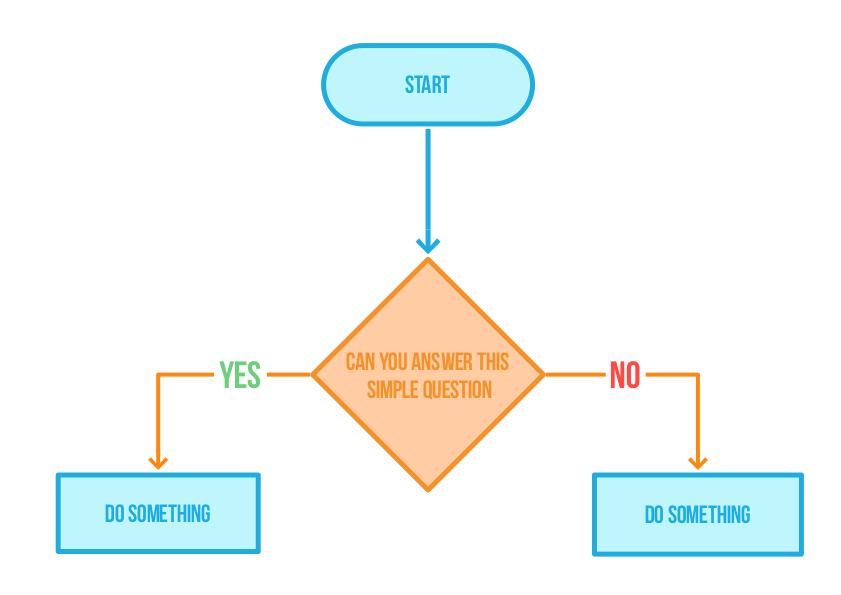
\includegraphics[scale=0.5]{figures/Flowchart}
    \caption{Caption for flowchart}
  	\medskip 
	\hspace*{15pt}\hbox{\scriptsize Credit: Acme company makes everything \url{https://acme.com/}}
    \label{FlowchartFigure}
\end{figure}

\subsection{Tables}

We can also do tables. Protip: use \url{https://www.tablesgenerator.com/} for generating tables.
\begin{table}[H]
\centering
\caption{Caption of table}
\label{TableLabel}
\begin{tabular}{|l|l|l|}
\hline
Title1 & Title2 & Title3 \\ \hline
data1  & data2  & data3  \\ \hline
\end{tabular}
\end{table}

\subsection{\gls{git}}

\gls{git} is fun, use it!

\chapter{Background}
In this chapter, the field of cryptology will be introduced, with an emphasis on digital signatures and cryptanalysis.  
We also introduce some necessary facts and notions related to linear algebra and lattices, as well as probability theory and distributions.
Lastly, we introduce the notion of \textit{Gradient Search} and ADAM-optimizers, which will be a central tool in this thesis.

\section{Cryptology}
For this section, \cite{KL20} will be used.
\subsection{Cryptography}
\subsection{Cryptanalysis}

\section{Digital Signatures}
\subsection{Hash-and-Sign}
\subsection{GGH}
\subsection{NTRU}
\section{Algebra}
\subsection{Polynomials}
\subsection{Polynomial rings}
\subsection{Number fields}
\section{Linear Algebra and Lattices}
Denote by $\vec{v}$ an $n \times 1$ column vector on the form 
\[ \vec{v} = \begin{bmatrix} v_0 \\ v_1 \\ ... \\ v_{n-1} \end{bmatrix}\] and by $\mat{B}$ an $n \times m$ matrix on the form 
\[
    \mat{B} = 
    \begin{bmatrix}
        b_{0,0} & b_{0,1} & \cdots & b_{0, n-1} \\ 
        b_{1,0} & b_{1,1} & \cdots & b_{1, n-1} \\ 
        \cdots & \cdots & \cdots & \cdots\\
        b_{m-1,0} & b_{m-1,1} & \cdots & b_{m-1, n-1} \\ 
    \end{bmatrix}
\]

Generally, entries $v_i$ and $b_{i, j}$ are integers unless stated otherwise.
Some places the thesis will use row notation instead of column notation for the vectors, so that $\vec{v}$ is a $1 \times n$ row vector on the form
\[\vec{c} = [v_0, v_1, ..., v_{n-1}]\] In these cases this will be pointed out.

We denote by $\langle \cdot, \cdot \rangle$ the dot-product of two vectors of equal dimensions as \\
$\langle \vec{x}, \vec{y} \rangle = \vec{x}^t \vec{y} = \mathlarger{\sum_{i=0}^{n-1} x_i y_i}$
\section{Probability Theory}
\section{Gradient Search}

\chapter{Hawk and HPP}
\section{Overview}
In this chapter, the Hawk digital signature scheme and the \textit{Learning a Parallelepiped} cryptanalytic attack will be presented.
This will lay the foundation for chapter 4, which will employ the \textit{Learning a Parallelepiped} attack against Hawk

In section 3.2, an introduction on how Hawk works on a high level will be given. The algorithms for key generation, signature 
generation and verification and their most important subroutines will be provided with enough detail in order to analyze them properly.
Section 3.3 will discuss some considerations for implementing the scheme.
The \textit{Learning a Parallelepiped} attack is described in section 3.4.

\section{Hawk}
In this section we introduce the digital signature scheme Hawk, which will later be the target for our cryptanalysis.
As mentioned in the introduction, Hawk is a lattice based signature scheme that shares some key points with that of NTRU-sign \cite{HHPSW03}.
Perhaps the most notable similarity is the algebraic structure of private key $\mat{B}$. Recall that in NTRU, polynomials are defined 
over $\bb{Z}[X] / (X^n - 1)$, whereas in Hawk they are defined over $\bb{Z}[X] / (X^n + 1)$.
% The private key in NTRU is defined as 
% \[
%     \begin{bmatrix}
%         f_0 & f_1 & \cdots & f_{n-1} & g_0 & g_1 & \cdots & g_{n-1} \\
%         f_{n-1} & f_{0} & \cdots & \cdots & g_{n-1} & f_{0} & \cdots \\
%         \cdots \\ 
%         f_{1} & f_{2} & \cdots & f_{n-1} & f_0 & g_{1} & g_{2} & \cdots & g_{n-1} & g_0 \\
%         F_0 & F_1 & \cdots & F_{n-1} & G_0 & G_1 & \cdots & G_{n-1} \\
%         F_{n-1} & F_{0} & \cdots & \cdots & G_{n-1} & F_{0} & \cdots \\
%         \cdots \\ 
%         F_{1} & F_{2} & \cdots & F_{n-1} & F_0 & G_{1} & G_{2} & \cdots & G_{n-1} & G_0 \\
%     \end{bmatrix}
% \]
\subsection{Overview}
In Hawk, polynomials are defined over the cyclotomic number field $\mathcal{K}_n = \bb{Q}[X]/(X^n +1)$ which has the corresponding ring of integers
$\bb{Z}[X] / (X^n + 1)$.
\subsection{Hawk key pairs and key pair generation}
A Hawk private key is represented by the $2 \times 2$ matrix.
\[ \mat{B} = 
    \begin{bmatrix} 
        f & F \\
        g & G
    \end{bmatrix} 
\]
\subsection{Hawk signature generation}
\subsection{Hawk signature verification}
\subsection{Hawk security}
\section{Implementation of Hawk}


\newcommand{\PP}[2][]{\mathcal{P}_{#1}(\mat{#2})}
\newcommand{\mat}[1]{\mathit{#1}}
\renewcommand{\vec}[1]{\mathbf{#1}}
\newcommand{\GLnR}{\mathcal{GL}_{n}(\mathbb{R})}
\newcommand{\normdist}[2]{\mathcal{N}(#1, #2^2)}
\newcommand{\dgdist}{\mathcal{D}_{2\bb{Z}+c, \sigma}}
\newcommand{\bb}[1]{\mathbb{#1}}

\newtheorem{lemma}{Lemma}
\newtheorem{proof}{Proof}

\section{HPP}
\section{HPP against the Normal Distribution}

\begin{lemma}[Lemma 1]
\label{hpp_norm_lemma}
Assume signatures on the form $\vec{v} = \vec{x} \mat{V}$ where $x_i \sim \normdist{0}{\sigma}$. After converting $\PP{V}$ to $\PP{C}$, the fourth moment of $\PP{C}$ is constant over some $\vec{w}$ on the unit circle.
% \in \mathcal{O}](\bb{R})$
\end{lemma}
\begin{proof}
    Some proof here
\end{proof}

\chapter{Cryptanalysis of Hawk}

\section{Overview}
In this chapter we introduce our cryptanalysis of Hawk by adapting the original HPP attack to the Hawk setting.
As previously shown, a continuous normal distribution is immune against such an attack due to the constant 4-th moment. In Hawk, however, the distribution of $\vec{x}$ is discrete, not continuous.
We will show in section 4.2 that the Discrete Gaussian Distribution based on tables and the algorithm \ref{sample} is indeed not identical to a continuous normal distribution, and that an attack akin to the original HPP may still be applicable.

In section 4.3, we explain the procedure to transform the hidden parallelepiped to a hidden hypercube, and show why this is a trivial task for Hawk signatures.
Section 4.4 will cover the main part of the attack, namely the gradient descent, which will in many ways be similar to the original attack.
Lastly, section 4.5 will present the complete practical method and give details about its implementation.

\section{Redefining the problem}

We now redefine the hidden parallelepiped problem in the Hawk setting.
Recall in HPP that one observes $\vec{v} = \mat{V} \vec{x}$. In the Hawk setting, the observed signature is $\vec{w} = \mat{B}^{-1} \vec{x}$. 
The problem now becomes: \\
Given signature samples on the form $\vec{w} = \mat{B}^{-1} \vec{x}$ where only $\vec{w}$ is known, $\mat{B}$ is a Hawk private key and $\vec{x}$ is distributed according to the discrete Gaussian Distribution $\dgd_{2\bb{Z}^{2n} + \vec{t}, \sigma}$,
recover columns of $\mat{B}$.
The general steps in Hawk setting will be similar to that of the original HPP:
\begin{itemize}
    \item Compute Covariance Matrix $(\mat{B}^{-1})^T (\mat{B}^{-1})$
    \item Transform the samples $\vec{w} \in \PP{\mat{B}^{-1}}$ to $\vec{c} \in \PP{C}$ where $\mat{C}$ is orthonormal
    \item Deduce columns of $\mat{C}$ doing gradient descent of minimizing the 4th moment of one-dimensional projections of $\PP{C}$
\end{itemize}


Assume observed signatures on the form $\vec{c} = \mat{C} \vec{z}$ where $\mat{C}$ is orthonormal (columns are unit vectors and pairwise orthogonal). 
Note that in this section we denote by $\vec{u}$ a vector on the unit sphere $\bb{R}^{2n}$ instead of $\vec{w}$ as in the previous section, to avoid confusion with the Hawk notation for $\vec{w} = \mat{B}^{-1} \vec{x}$.
Also note that henceforth we will consider only $\vec{w} = \mat{B}^{-1} \vec{x}$ as a signature instead of $\vec{s} = \frac{1}{2}(\vec{h} - \vec{w})$ since $\vec{w}$ is easily recoverable given $\vec{s}$ and message $\vec{m}$.
Lastly, we consider $\mat{B}$ as $\mathsf{rot}(\mat{B})$ and thus work with matrices in $\bb{Q}^{2n \times 2n}$ and vectors in $\bb{Q}^{2n}$ in this section. \todo{Explain a bit better $\bb{Q}$ vs $\bb{Z}$ for completeness.}

By rewriting the terms from the original HPP paper \cite{NR09} for this new, normalized, distribution $\dgdi$, we have that
\[mom_{4, \mat{C}} (\vec{u}) = 3 \lVert \vec{u} \rVert ^4 + (\mu_4 - 3) \sum_{i=1}^{n} \langle c_i, \vec{u} \rangle^4 \]
and
\[\nabla mom_{4, \mat{C}} (\vec{u}) = 12 \lVert \vec{u} \rVert^2 \vec{u} + 4(\mu_4 - 3) \mathlarger{\sum_{i=1}^{n} \langle c_i, \vec{u}} \rangle^3 c_i\]
where $\vec{u}$ is a vector on the unit sphere of $\bb{R}^{2n}$, i.e. $\lVert \vec{u} \rVert = 1$. 
% \footnote{Note that in the previous chapter about HPP, $\vec{w}$ was used to denote a vector on the unit sphere of $\bb{R}^{2n}$.
% Here we denote by $\vec{u}$ such a vector as to not confuse it with our current meaning of $\vec{w}$, which denotes a signature $\vec{w} = \mat{B}^{-1} \vec{x}$}
This means that if the difference $(\mu_4 - 3)$ is significant enough, one might be able to employ the same minimization technique as in the original attack to reveal a column of $\mat{C}$ 
because $\langle c_i, \vec{u} \rangle^4 = 1$ if $\vec{u} = \pm c_i$ since $\langle c_i, c_i \rangle^4 = 1$.
Note that if $(\mu_4 - 3) < 0$ we have the same case as in the original attack, where minimization of the entire term entails maximization of $\mathlarger{\sum_{i=1}^{n} \langle c_i, \vec{u} \rangle^4}$, which gives us a row of $\pm \mat{C}$.
If $(\mu_4 - 3) > 0$, we need to maximize the entire term $3 \lVert \vec{u} \rVert ^4 + \mathlarger{\sum_{i=1}^{n} \langle c_i, \vec{u} \rangle^4}$, which is achieved by doing a gradient \textit{ascent} instead of a gradient \textit{descent}.

\section{Estimating $\mu_4$}


\subsection{Estimating $\mu_4$ via direct sampling}
Consider the Discrete Gaussian Distribution as described in \cite{HawkSpec24} and section 3.1.5. We can use our implementation of Hawk to sample many points from the distribution.
Let $\dgdi$ denote the practical discrete Gaussian distribution from sampled points.
Let $\hat{\mu}$, $\hat{\sigma}^2$ be the expectation and variance of $\dgdi$.
Assume we sample $t$ points from $\dgdi$ as $X = \{x_1, x_2, ..., x_t\}$. We estimate $\hat{\mu}$ and $\hat{\sigma}^2$ simply as $\hat{\mu} = \mathlarger{\frac{1}{t} \sum_{i=1}^{t} x_i}$ and $\hat{\sigma}^2 = \mathlarger{\frac{1}{t} \sum_{i=1}^{t}(x_i - \hat{\mu})^2}$.
For simplicity, we can also assume $\hat{\mu} = 0$ as claimed in \cite{HawkSpec24}.
To simplify later computations we also normalize our samples by computing $Z = \{z_1, z_2, ..., z_t\} = \{\frac{x_1}{\hat{\sigma}}, \frac{x_2}{\hat{\sigma}},..., \frac{x_t}{\hat{\sigma}}\}$ such that 
$\bb{V}[z_i] = 1$.
Now $\hat{\mu}_4 = \bb{E}[z_i^4] = \mathlarger{\frac{1}{t} \sum_{i=1}^{n} z_i ^4}$. 

The problem with this approach is the requirement of many samples in order to determine $\hat{\mu}_4$ with high enough accuracy.
By using Confidence Intervals and Central Limit Theorem, we get a number of how many samples one should sample in order for $\hat{\mu}_4$ to be accurate.

\[
    n = (\frac{z_{\alpha / 2} \cdot \hat{\sigma}}{E} )^2    
\]
where $E$ is the acceptable error and $z_{\alpha / 2}$ is found in standard normal tables.
Assume one wants to determine with confidence $95 \%$ that an estimate $\hat{\mu}_4$ differs from the real $\mu_4$ by maximum $0.00001$, or $1 \times 10^{-5}$.
Then $n = (\frac{1.96 \cdot \hat{\sigma}} {10^{-5}})^2$
\todo{Show this value maybe??}

\subsection{Computing $\mu_4$ analytically}
The probability that one can discern $mom_{4, \mat{C}}(\vec{u})$ when $\vec{u} \in \pm \mat{C}$ and when $\vec{u} \not\in \pm \mat{C}$ ultimately depends on the value of $\mu_4$ and the number of signature samples one has available.
% If we can upper estimate the variance of $mom_{4, \mat{C}}(\vec{u})$ and $\nabla mom_{4, \mat{C}}(\vec{u})$ one can get an idea of how many samples one needs to do this distinguishment.

For implementation of Hawk, they provide tables which along with an algorithm determines the distribution $\dgdi_{2\bb{Z} + c, \sigma}$. Based on the tables one can reconstruct a 
Probability Mass Function (PMF) $Pr(X = x)$ for $X \sim \dgdi_{\bb{Z}, \sigma$.
    The PMF of $\dgdi_{\bb{Z}, \sigma$ from tables is:
\[
    Pr(X=x) = \frac{1}{2} \cdot
\begin{cases}
    1 - T_c[0] & \text{, if } \lvert x \rvert = c \\
    \frac{1}{2}\mathlarger{(T_c[\frac{\lvert x \rvert - c}{2} - 1] - T_c[\frac{\lvert x \rvert - c}{2}])} & \text{, if } \lvert x \rvert > c
\end{cases}
\]
Here, $c = \lvert x \rvert \mod{2}$ that determines which table ($T_0$ or $T_1$) is used. \todo{Explain this stuff a bit better maybe}

Given the PMF we can compute the moments of $X$ as $\bb{E}[X^k] = \mathlarger{\sum_x x^k \cdot Pr(X = x)}$, as there is a finite number of entries in the tables.
More specifically, for the 256 parameter set, there are 10 entries in $T_0$ and $T_1$. Therefore we sum from $x = -20$ to $x = 20$.
When $|x| = 20$, $Pr(\lvert X \rvert \geq 20) = \frac{1}{4} \cdot (T_0 [9] - T_0[10])$, where $T_0[9]$ is the last non-zero entry, and so all successive entries will yield 0.
Similarly, for parameters 512 and 1024 we sum from $x = -26$ to $x = 26$, since there are 13 entries in $T_0$ and $T_1$.

By using the Decimal module in Python \cite{Decimal}, a module designed for high precision when working with decimal numbers, we can be confident that the computed results are correct, 
and that we do not get e.g. floating point errors when summing, since we are dealing with very small numbers.

We compute $\mu_4$ as $\mu_4 = \bb{E}[Z^4] = \bb{E}[(\frac{X}{\sigma})^4] = \frac{1}{\sigma^4}\bb{E}[X^4]$.
In table \ref{z4 values} we show the value of $\mu_4$ and $\mu_4 - 3$ rounded at 25 and 39 decimal points, respectively, for all three Hawk degrees.

\begin{table}[H]
    \centering
    \caption{Measure of $\mu_4$}
    \label{z4 values}
    \begin{tabular}{lcc}
        \toprule
        \textbf{Degree} & $\bb{E}[Z^4]$ & $\bb{E}[Z^4] - 3$ \\
        \midrule
        256 & 2.9999999999999790015752619 & -2.0998424738064930232320331 $\cdot 10^{-14}$ \\
        \midrule
        512 & 2.9999999999999999999862684 & -1.3731593731486976093589903 $\cdot 10^{-20}$ \\
        \midrule
        1024 & 2.999999999999999999987558 & -1.2441396421557256288414318 $\cdot 10^{-20}$ \\
        \bottomrule
    \end{tabular}
\end{table}

Using this measure we can estimate how many samples we need for $\mu_4 - 3$ to be detectable.
We use the following equation from using the Central Limit Theorem (CLT): 
\[
    n \geq (\frac{z\cdot \sigma}{\mathsf{err}})^2
\]

\section{Covariance matrix and hypercube transformation}
In the original HPP attack one has to estimate the matrix $\mat{G} \approx \mat{V} ^t \mat{V}$.
For Hawk, the signatures are on the form $\vec{w} = \mat{B}^{-1} \vec{x}$. Then we would need to compute $\mat{G} = \mat{B}^{-1} \mat{B}^{-T}$ (the HPP paper uses row vectors while Hawk use columns vectors).
However, the public key $\mat{Q} = \mat{B}^T \mat{B}$, enables us to skip this step.
Recall that in the original attack one has to take Cholesky decomposition (or an equivalent decomposition) of the inverse of the covariance matrix such that $\mat{G}^{-1} = \mat{L}\mat{L}^T$. 
For $\mat{G} = \mat{B}^{-1} \mat{B}^{-T}$, the inverse,
$\mat{G}^{-1} = \mat{B}^T \mat{B} = \mat{Q}$. Therefore, we can simply take the Cholesky decomposition of $\mat{Q}$ to get $\mat{L} \text{ such that } \mat{Q} = \mat{L} \mat{L}^T$.
By multiplying our samples $\vec{w}$ by $\mat{L}^T$ on the left, we have transformed our samples to the hidden hypercube as in the original attack. \\
By taking $\mat{C} =  \mat{L}^T\mat{B}^{-1}$, we have that 
\[\mat{C}^T \mat{C} = (\mat{L}^T \mat{B}^{-1})^T (\mat{L}^T \mat{B}^{-1}) = \mat{B}^{-T} \mat{L} \mat{L}^T \mat{B}^{-1} = \mat{B}^{-T} \mat{Q} \mat{B}^{-1} = \mat{B}^{-T} \mat{B}^{T} \mat{B} \mat{B}^{-1} = \mat{I}_n\]
and
\[\mat{C}\mat{C}^T = (\mat{L}^T \mat{B}^{-1})(\mat{L}^T \mat{B}^{-1})^T = \mat{L}^T \mat{B}^{-1} \mat{B}^{-T} \mat{L} =  \mat{L}^T \mat{Q}^{-1} \mat{L} = \mat{L}^T (\mat{L} \mat{L}^T)^{-1} \mat{L} = \mat{L}^T \mat{L}^{-T} \mat{L}^{-1} \mat{L} = \mat{I}_n\]
Thus $\mat{C}$ is an orthonormal matrix.
Since $\vec{w}$ is distributed according to $\dgdi$ over $\PP{\mat{B}^{-1}}$, by taking 
$\vec{c} = \mat{L}^{T} \vec{w}$ we have $\vec{c} = \mat{L}^{T} \mat{B}^{-1} \vec{x} = \mat{C} \vec{x}$, $\vec{c}$ is distributed according to $\dgdi$ over $\PP{C}$.

We summarize this step of the attack against Hawk in the following algorithm

\begin{algorithm}
\caption{Hawk Hypercube Transformation}
\begin{algorithmic}[1]
% \Procedure{Euclid}{$a,b$}\Comment{The g.c.d. of a and b}
    \Require{Samples $\vec{w} = \mat{B}^{-1} \vec{x}$ and public key $\mat{Q}$}
    \State Compute $\mat{L}$ s.t. $\mat{Q} = \mat{L}\mat{L}^T$ \Comment by Cholesky decomposition
    \State Compute $\vec{c} = \mat{L}^T \vec{w}$
    \State \Return{$\vec{c}$ and $\mat{L}^{-T}$}
\end{algorithmic}
\end{algorithm}

\section{Gradient search overview}

Now, given samples $\vec{c} \in \PP{C}$, we run a gradient search to minimize or maximize the fourth moment of one-dimensional projections onto $\vec{u}$, as in the original attack. In addition to multiplying the samples by $\mat{L}^T$, we also divide them by the scalar $\sigma$, to normalize the samples
so their variance is $1$. This also aligns with our theoretical analysis of $mom_{4,\mat{C}}(\vec{u})$. Even though the distribution $\dgdi$ is discrete, the shape of the samples $\vec{c} \in \PP{C}$ will still have a somewhat spherical shape,
as illustrated in figures \ref{parallelepiped_normal_discrete} and \ref{hypercube_normal_discrete}.
The hope is that the areas in the directions of the columns of $\pm \mat{C}$ will deviate just enough from a perfect spherical shape to give us a clear global minima/maxima in the gradient landscape.

We evaluate the functions $mom_{4, \mat{C}}(\vec{u})$ as $\bb{E} [\langle \vec{c}, \vec{u} \rangle ^4]$ and $\nabla mom_{4,\mat{C}}(\vec{u})$ as $\bb{E} [\nabla \langle \vec{c}, \vec{u} \rangle ^4] = 4 \bb{E} [\langle \vec{c}, \vec{u} \rangle ^3 \vec{c}]$.
These can be evaluated by precomputed samples $\{\vec{c}_1, \vec{c}_2, ..., \vec{c}_t\}$, or by continuously generating one and one signature sample since we have access to the signature generation algorithm.

\todo{This might be redundant, as the method will be described in chapter on HPP}
% Below, gradient descent adapted to is described as an algorithm, similar to . Note that the only difference is in what direction to move and the condition for termination, on lines 4 and 6 respectively.
\begin{algorithm}[H]
    \caption{Gradient descent on $\PP{C}$}
\begin{algorithmic}[1]
    \Require{Samples on the form $\vec{c} = \mat{C}\vec{x}$, descent parameter $\delta$}
    \State $\vec{u} \gets \text{ random vector on unit sphere in } \bb{R}^{2n}$
    \Loop
    \State $\vec{g} \gets \nabla \mom{4}{C}$
    \State $\vec{u}_{new} = \vec{u} - \delta \vec{g}$
    \State normalize $\vec{u}_{new}$ as $\frac{\vec{u}_{new}}{\lVert \vec{u}_{new} \rVert}$
    \If{$mom_{4, \mat{C}}(\vec{u}_{new}) \geq mom_{4, \mat{C}(\vec{u})}$}
    \State \Return{$\vec{u}$}
    \Else 
    \State $\vec{u} \gets \vec{u}_{new}$
    \State go to step 3
    \EndIf
    \EndLoop
\end{algorithmic}
\end{algorithm}

For a gradient \textit{ascent} one can flip the sign and inequality sign on lines 4 and 6, respectively.

\begin{figure}[H]
    \centering
    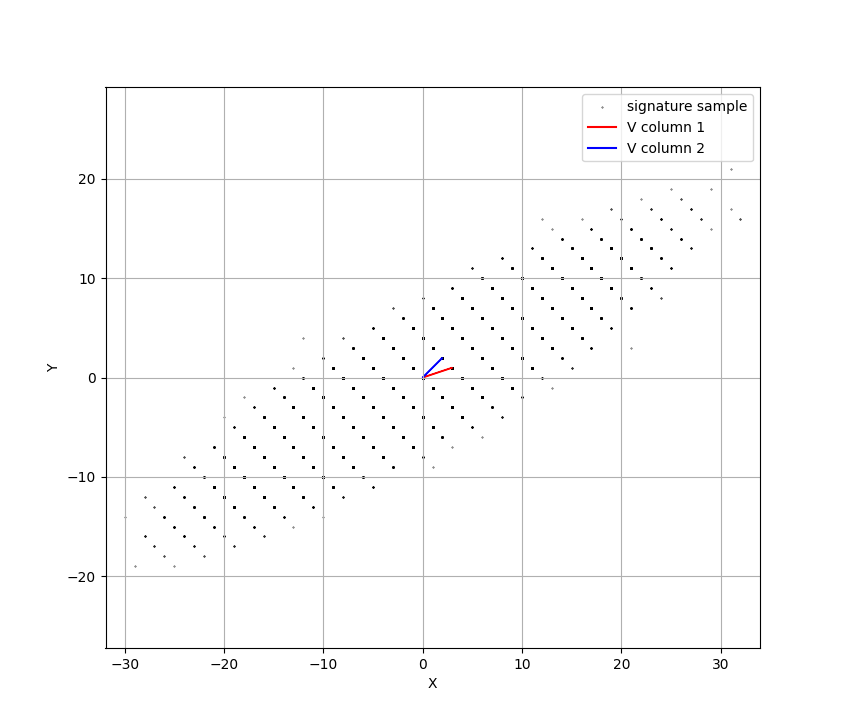
\includegraphics[scale=0.7]{hpp_parallelepiped_normal_discrete.png}
    \caption{Hidden parallelepiped in dimension 2 for discrete Gaussian distribution ($\sigma = 2.02$)}
  	\medskip 
	% \hspace*{15pt}\hbox{\scriptsize Credit: Acme company makes everything \url{https://acme.com/}}
    \label{parallelepiped_normal_discrete}
\end{figure}

\begin{figure}[H]
    \centering
    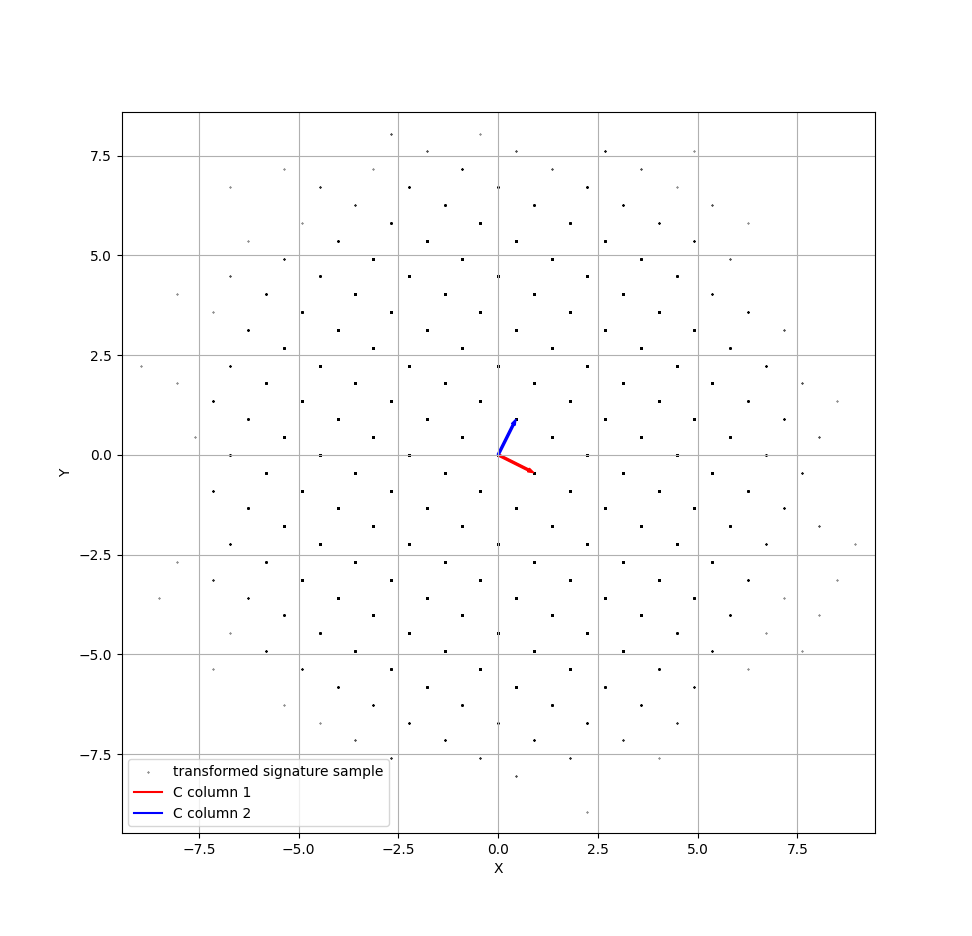
\includegraphics[scale=0.6]{hppnormal_cube_discrete.png}
    \caption{Hidden hypercube in dimension 2 for discrete Gaussian distribution ($\sigma = 2.02$)}
  	\medskip 
	% \hspace*{15pt}\hbox{\scriptsize Credit: Acme company makes everything \url{https://acme.com/}}
    \label{hypercube_normal_discrete}
\end{figure}
\section{Practical method}

Below is a basic description of the approach.
\begin{algorithm}[H]
\caption{Proposed basic version of attack}
\begin{algorithmic}[1]
    \State Collect signatures $\vec{w} = \mat{B}^{-1} \vec{x}$
    \State Using public key $\mat{Q}$, find $\mat{L}$ s.t. $\mat{Q} = \mat{L} \mat{L}^T$
    \State Transform samples s.t. $\vec{c} = \mat{L}^T \vec{w}$
    \State Find columns of $\pm \mat{C}$ by doing gradient search over $\PP{C}$
    \State Multiply columns of $\pm \mat{C}$ by $\mat{L}^{-T}$ on the left and round the result to get columns in $\pm \mat{B}^{-1}$
\end{algorithmic}
\end{algorithm}

After having transformed the samples $\vec{w} \in \PP{\mat{B}^{-1}}$ to $\vec{c} \in \PP{\mat{C}}$ we want to recover columns of $\pm \mat{C}$ and transform them back to columns of $\pm \mat{B}^{-1}$ by multiplying by $\mat{L}^{-T}$ on the left.
Due to the special structure of Hawk private keys, finding one column of $\mat{B}$ automatically gives $n$ columns.
Unfortunately, since revealing a single column of $ \mat{B}^{-1}$ reveals a "shift" of either the two polynomials $G$ and $ g$ \textit{or} $F$ and $f$,
this is not enough to disclose the entire matrix. If samples were on the form $\vec{w} = \mat{B} \vec{x}$, a single column would reveal $f$ and $g$ (or $F$ and $G$), and one could simply reconstruct $F$ and $G$ (or $f$ and $g$)
by solving the NTRU-equation as in the key generation step of Hawk.
Nevertheless, if one finds two columns of $\mat{B}^{-1}$, it is easy to check if they are shifts of each other. If they are not, one has found shifts of all four polynomials in the secret key, 
and by trying all combinations of shifts, of which there are $4 n^2$ (accounting for negative and positive sign), one can easily verify if a candidate $\mat{B'}$ is valid by 
checking if $\mat{B}'$ is unimodular and if $\mat{B'}^T \mat{B'} = \mat{Q}$. If so, one is able to forge signatures, and the attack is done.

After each gradient ascent and/or descent returns a possible solution $\vec{z}'$, 
we multiply it to the left as $\vec{b}' = \mat{L}^{-T} \vec{z}'$ where $\vec{b}'$ is a possible column of $\pm \mat{B}^{-1}$ as $\vec{z}'$ is a possible column of $\pm \mat{C} = \mat{L}^T \cdot (\pm \mat{B}^{-1})$.
Since in experiments we have access to the correct secret key, we simply check directly if $\mat{b}' \in \pm \mat{B}^{-1}$.
In a real word attack however, one would, as described above, have to compute candidate $\mat{B}'$ and check if $\mat{B}'^T\mat{B}' = \mat{Q}$.

Having access to the correct $\mat{B}^{-1}$ we can do measures on how close a proposed solution $\vec{b}'$ is to one of the columns of $\mat{B}^{-1}$.
We can for example take the difference in length of $\lvert \vec{b}' \rvert $ and each vector in $\lvert \mat{B}^{-1}\rvert$, i.e. 
$ \mathsf{diff_{min}} = \mathsf{min} \{\lVert \lvert \vec{b}' \rvert - \lvert \vec{b}_i \rvert \rVert \ \mathbf{:} \ \vec{b}_i \in \pm \mat{B}^{-1}\}$.
A low value for this (this depends on the Hawk parameter $n$) would indicate a good guess, whereas a higher value indicates greater difference between the vectors, and thus a bad guess.
% One can also take the average of the difference of the entries in the vectors, i.e. $ \mathsf{diff_{min}} = \mathsf{min} \{\frac{1}{2n} | \vec{b}' - \vec{b}_i | \mathbf{:} \vec{b}_i \in \pm \mat{B}^{-1}\}$.
Alternatively, one can count entrywise how many entries out of $2n$ that matches between $\vec{b}'$ and $\vec{b}_i$, or use some other suitable measurement.

A concern about this approach of attacking Hawk is the gradient search, as described in Algorithm 2 and 3. In the original HPP attack, they used a standard gradient descent with a constant stepsize/descent parameter $\delta$. This
worked fine for attack on GGH and NTRU when the global minima (of which there are $2n$) of the gradient landscape was very obvious. In the gradient landscape of Hawk however, there is much more noise, and the global minima is
not as clear, as it depends on the discrepancy $(\mu_4 - 3)$, which is quite small. Generally, a constant stepsize $\delta$ entails a tradeoff between slow convergence and the risk of "overshooting" the correct global extremum.  
We therefore employ the method of ADAM-optimizer, as described in chapter 2.
Below is a description of the gradient search using ADAM-optimizer in our setting.

\begin{algorithm}[H]
    \caption{$\mathsf{gradient \ descent \ ADAM}$}
\begin{algorithmic}[1]
    \Require{signatures $\vec{c} = \mat{C} \vec{x}$}
    \Require{Stepsize $\delta$, decay rates $\beta_1, \beta_2$}
    \State $\vec{u} \gets $ random vector on the unit sphere of $\bb{R}^{2n}$
    \State $\vec{m}_0 \gets 0$ \Comment{Vector of 0's}
    \State $\vec{v}_0 \gets 0$ \Comment{Vector of 0's}
    \State $t \gets 0$ \Comment{Timestep}
    \Loop
    \State $t \gets t + 1$
    \State $\vec{g}_t \gets \nabla mom_{4, \mat{C}}(\vec{u})$
    \State $\vec{m}_t \gets \beta_1 \cdot \vec{m}_{t-1} + (1 - \beta_1) \cdot \vec{g}_t$
    \State $\vec{v}_t \gets \beta_2 \cdot \vec{v}_{t-1} + (1 - \beta_2) \cdot \vec{g}_t^2$
    \State $\hat{\vec{m}}_t \gets \vec{m}_t / (1 - \beta_1 ^t) $
    \State $\hat{\vec{v}}_t \gets \vec{v}_t / (1 - \beta_2 ^t) $
    \State $\vec{u}_{new} \gets \vec{u} - \delta \cdot \hat{\vec{m}}_t / (\sqrt{\hat{\vec{v}}_t + \epsilon})$ \Comment{Flip the $-$ sign for gradient ascent}
    \State normalize $\vec{u}_{new}$ as $\frac{\vec{u}_{new}}{\lVert \vec{u}_{new} \rVert}$
    \If{$mom_{4, \mat{C}}(\vec{u}_{new}) \geq mom_{4, \mat{C}}(\vec{u})$} \Comment{Flip the $\geq$ sign for gradient ascent}
    \State \Return{$\vec{u}$}
    \Else 
    \State $\vec{u} \gets \vec{u}_{new}$
    \State go to step 6
    \EndIf
    \EndLoop
\end{algorithmic}
\end{algorithm}

The $\epsilon$ in step 12 of the algorithm is inserted to not divide by 0. Proposed value for $\epsilon = 10^{-8}$,
and proposed good values for $\delta, \beta_1$ and $\beta_2$ are $0.001, 0.9$ and $0.999$ respectively.
In this method, the stepsize then depends on $\delta, \vec{m}_t$ and $\vec{v}_t$.
Explanation of variables:
\begin{itemize}
    \item $\vec{m}_t$ estimates an average of previous gradients, as to make movement in one iteration partially depend on the direction of previous iterations.
    \item $\vec{v}_t$ estimates the variance of the previous gradients. Larger variance will reduce the stepsize to not overshoot possible extremum, while lower variance will increase the stepsize to speed up convergence.
    \item $\hat{\vec{m}}_t$ and $\hat{\vec{v}}_t$ is bias-correction, so that the first iterations are not biased towards 0.
\end{itemize}
\todo{This should be in the theoretical background}

Below is a more detailed version of the entire attack/experiment.
\begin{algorithm}[H]
\caption{Proposed version of attack with measuring}
\begin{algorithmic}[1]
    \Require{Hawk parameter $n$, number of samples $t$, Hawk key pair $\mat{B}$, $\mat{Q}$}
    \State Collect $t$ signatures $\vec{w} = \mat{B}^{-1} \vec{x}$ \Comment{Optional - can also generate signatures continuously}
    \State Using public key $\mat{Q}$, compute $\mat{L}$ s.t. $\mat{Q} = \mat{L} \mat{L}^t$
    \State Transform samples s.t. $\vec{c} = \mat{L}^t \vec{w}$
    \Loop
    \State Candidate $\vec{z}' \gets \mathsf{gradient \ search  \ ADAM}$ \Comment{Do both ascent and descent}
    \State Candidate $\vec{b}' \gets \lfloor \mat{L}^{-T} \vec{z}' \rceil$ \Comment{Entrywise rounding to nearest integer}
    \State Check if $\vec{b}' \in \mat{B}^{-1}$
    \State Measure $\mathsf{diff_{min}}(\vec{b}', \mat{B}^{-1})$
    \EndLoop
\end{algorithmic}
\end{algorithm}

The loop from line 4 can be run several times to get a new random starting point $\vec{u}$ for the gradient search.
Line 6 rounds the candidate \textit{after} multiplying with $\mat{L}^{-T}$ to avoid rounding errors.
Line 8 can also give which column of $\mat{B}^{-1}$ $\vec{b}'$ is closest to, so one can compare the vectors side by side.

\section{Results}

The method has unfortunately not proven to work, as no correct key has been found in any of the runs. It seems that regardless of number of signatures (above a certain point, e.g. one million), the method cannot give candidate solutions with
better comparison than random guessing. Random guessing in this case is assuming one knows what type of distribution the columns of a secret key is. One knows the distribution that $f, g$ follows, but $F$ and $G$ depends on $f$ and $g$.

For reference, I ran a test using the closeness measure $ \mathsf{diff_{min}} = \mathsf{min} \{\lVert \lvert \vec{b}' \rvert - \lvert \vec{b}_i \rvert \rVert \ \mathbf{:} \ \vec{b}_i \in \pm \mat{B}^{-1}\}$ by fixing one private key $(\mat{B}^{-1})$, 
and generating random keys $\mat{B}^{'-1}$ (which will serve as random guesses), to check if the attack on average gives better results than random
guessing. Table 1 shows the result of comparing a key with 100 random keys, and the result of 100 random starting points for the gradient search (both ascent and descent).

One thing to note is that Hawk does not specify parameters (such as width $\sigma$ of $\dgdi$) for lower values of $n$ than 256. Therefore, when sampling signatures for $n=32, 64$ and $128$, I use the same tables, i.e. same $\sigma$ for $\dgdi$, as in Hawk 256.

\begin{table}[H]
    \centering
    \caption{Closeness measure for Hawk attack}
    % \label{tab:hawk-parameters}
    \begin{tabular}{lcccc}
        \toprule
        \textbf{Type} & $\mathsf{diff_{min}}$ & $\mathsf{diff_{max}}$ & \textbf{Avg $\mathsf{diff_{min}}$} & \textbf{Avg $\mathsf{diff_{max}}$} \\
        \midrule
        Key comparison degree 32 & 6.25 & 15.81 & 7.74 & 11.22 \\
        Attack on Hawk 32 (1m samples) & 7.14 & 16.24 & 8.50 & 12.87 \\
        \midrule
        Key comparison degree 64 & 10.77 & 26.51 & 13.96 & 22.18 \\
        Attack on Hawk 64 (1m samples) & 13.49 & 26.00 & 16.25 & 22.59 \\
        \midrule
        Key comparison degree 128 & 25.33 & 47.26 & 30.00 & 41.60 \\
        Attack on Hawk 128(1m samples) & 24.27 & 46.91 & 29.61 & 46.91 \\
        \midrule

        Key comparison degree 256 & 56.33 & 82.34 & 61.02 & 75.02 \\
        Attack on Hawk 256 (1m samples) & 54.50 & 84.07 & 59.20 & 71.09 \\ 
        Attack on Hawk 256 (10m samples) & 57.72 & 77.54 & 62.37 & 77.54 \\
        \bottomrule
    \end{tabular}
\end{table}
Lastly, I include values from sampling points from $\dgdi$ for Hawk 256. 100 million vectors $\vec{x}$ were sampled, resulting in $2 \cdot 256 \cdot 100$ million independently sampled points from $\dgdi$.
First, I compute $\sigma^2$ and $\sigma$, then compute $\mu_4$ of normalized samples on the form $z = \frac{x}{\sigma}$.
We then get that 
\begin{itemize}
    \item $\sigma^2 = 4.080429335$
    \item $\sigma = 2.020007261$
    \item Normalized $\mu_4 = \bb{E} (z^4) = 3.000007624$
    \item $(\mu_4 - 3) = 0.000007624$
\end{itemize}

\section{Conclusion}
In conclusion, I think the reason the method has not worked is because of the small value of $(\mu_4 - 3)$, but importantly also because of the noisy nature of the distribution $\dgdi$. 
The noise introduces too many "false" local minima/maxima in the gradient landscape such that it is difficult to find the correct \textit{global} minima/maxima.
I do not claim that it is impossible, but my experiments show that it seems infeasible for this particular approach.


% Include more chapters as required.
%%=========================================

% Alternative 1 of printing glossaries & acronyms
%\renewcommand{\glossarypreamble}{\footnotesize}
%\printglossary[style=super, type=\glsdefaulttype] \let\cleardoublepage\clearpage
%\printglossary[style=super, type=\acronymtype]


%Alternative 2
%Simplified way of printing glossaries, slower than alt 1, but has better compatibility
\printnoidxglossaries

% Include more appendices as required.
%%=========================================
\clearpage
\DeclareRobustCommand{\VAN}[3]{#3}
\addcontentsline{toc}{chapter}{Bibliography}
\bibliographystyle{generators/myplainnat}
\bibliography{generators/refs}
\appendix
\titleformat{\chapter}[display]
  {\normalfont\large\bfseries}% <- font for label "Appendix A", default \huge
  {\chaptertitlename\ \thechapter}
  {20pt}
  {\large}% <- font for title, default \Huge

\chapter{Generated code from Protocol buffers}

\begin{lstlisting}[caption={Source code of something},label=Listing]
System.out.println("Hello Mars");
\end{lstlisting}
\end{document}
